\documentclass[notes]{subfiles}
\begin{document}
	\addcontentsline{toc}{section}{12.4 - The Cross Product}
	\refstepcounter{section}
	\fancyhead[RO,LE]{\bfseries \nameref{cs124}} 
	\fancyhead[LO,RE]{\bfseries \small \currentname}
	\fancyfoot[C]{{}}
	\fancyfoot[RO,LE]{\large \thepage}	%Footer on Right \thepage is pagenumber
	\fancyfoot[LO,RE]{\large Chapter 12.4}
	
\section*{The Cross Product}\label{cs124}
	\subsection*{Before Class}
	\subsubsection*{The Cross Product}
		\begin{defn}[Cross Product (Algebraic Definition)]
			The \textbf{cross product} of two vectors $\textbf{a} = \lrangle{a_1,a_2,a_3}$ and $\textbf{b} = \lrangle{b_1,b_2,b_3}$ is defined to be the vector\\[15pt]
				\[\textbf{a}\times\textbf{b} = \hspace{4in}\]
		\end{defn}
		
		\begin{rmk}[Physical Meaning of the Cross Product]
			The cross product $\textbf{a}\times\textbf{b}$ produces a \blank{1.5} which is \blank{2} to both \textbf{a} and \textbf{b}
		\end{rmk}
		
		\begin{rmk}[Determinant of a $2\times 2$ Matrix]
			\[\left|\begin{matrix} a & b \\ c & d\end{matrix}\right| = \hspace{2in}\]
		\end{rmk}
		
		\begin{rmk}[Determinant of a $3\times 3$ Matrix]
			\[
				\left|\begin{matrix} a_1 & a_2 & a_3 \\ b_1 & b_2 & b_3 \\ c_1 & c_2 & c_3 \end{matrix}\right| = \hspace{4in}\]
				\\[15pt]
				%\[= \hspace{2.12in}\]
		\end{rmk}
			\newpage
			
		\begin{rmk}[The Cross Product as a Determinant]
			
			\[\textbf{a}\times \textbf{b} = \hspace{4.5in}\]
		\end{rmk}
			
		\begin{ex}
			If $\textbf{u} = \lrangle{1,4,3}$ and $\textbf{v} = \lrangle{5,-7,2}$, find the following:
			\begin{enumerate}[(a)]
				\item $\textbf{u}\times \textbf{v}$
					\vs{1}
					
				\item $(2\textbf{u})\times \textbf{v}$
					\vs{1}
					
				\item $\textbf{u}\times \textbf{u}$
					\vs{1}
					
				\item $\textbf{v}\times \textbf{u}$	
					\vs{1}
			\end{enumerate}
		\end{ex}
			\newpage
			
		\begin{defn}[Cross Product (Geometric Definition)]
			If $\theta$ is the angle between the vectors $\textbf{a}$ and $\textbf{b}$ (so that $0\leq \theta\leq \pi$), then\\[15pt]
				\[|\textbf{a}\times \textbf{b}| =\hspace{2in}\]
		\end{defn}
		
		\begin{question}
			What happens in the cross product if $\theta = 0$ or $\theta = \pi$?  Is there a geometric interpretation for this?
		\end{question}
			\vs{1}
			
		\begin{rmk}[Applications of the Cross Product]
			Let $\textbf{a}$ and $\textbf{b}$ be two nozero vectors.\\[15pt]
			\begin{itemize}
			\setlength\itemsep{15pt}
				\item \blank{3} if and only if \blank{2}.
				\item The value $|\textbf{a}\times\textbf{b}|$ is equal to \blank{3} determined by \textbf{a} and \textbf{b}.
			\end{itemize}
		\end{rmk}
		
		\begin{ex}
			Find a vector perpendicular to the plane that passes through the points $(1,4,5)$, $(-2,5,1)$, and $(1,-1,1)$.
		\end{ex}
			\vs{1}
			\newpage
			
	\subsection*{Pre-Class Activities}
		\begin{ex}
			Use this space to write any questions you might have from the videos.
		\end{ex}
			\vs{.5}
			
		\begin{ex}
			Compute the cross product of $\textbf{a}$ and $\textbf{b}$.
			\begin{enumerate}[(a)]
				\item $\textbf{a} = \lrangle{4,3,-2}$, $\textbf{b} = \lrangle{2,-1,1}$
					\vs{1}
					
				\item $\textbf{a} = \lrangle{3,3,-3}$, $\textbf{b} = \lrangle{3,-3,3}$
					\vs{1}
					
				\item $\textbf{a} = \lrangle{t,\cos t,\sin t}$, $\textbf{b} = \lrangle{1,-\sin t, \cos t}$
					\vs{1}
			\end{enumerate}
		\end{ex}
		
		\begin{ex}
			Find two unit vectors which are orthogonal to both $\lrangle{3,2,1}$ and to $\lrangle{-1,1,0}$
		\end{ex}
			\vs{1}
			
		\begin{ex}
			Find the area of the parallelogram with vertices $A(-3,0)$, $B(-1,3)$, $C(5,2)$, and $D(3,-1)$
		\end{ex}
			\vs{1}
			\newpage
			
	\subsection*{In Class}
		\begin{ex}
			Which of the following expressions are meaningful and which are meaningless?  Why?
		\end{ex}\\
		\begin{minipage}{7in}
			\begin{multicols*}{2}
				\begin{enumerate}[(a)]
					\setlength\itemsep{50pt}
					\item $\textbf{a}\cdot (\textbf{b}\times \textbf{c})$
					\item $\textbf{a}\times (\textbf{b}\times \textbf{c})$
					\item $(\textbf{a}\cdot \textbf{b})\times (\textbf{c}\cdot \textbf{d})$
						\columnbreak
					\item $\textbf{a}\times (\textbf{b}\cdot \textbf{c})$
					\item $\textbf{a}\cdot (\textbf{b}\cdot \textbf{c})$
					\item $(\textbf{a}\times\textbf{b})\cdot (\textbf{c}\times\textbf{d})$
				\end{enumerate}
					\raggedcolumns
			\end{multicols*}
		\end{minipage}
			\vs{.5}
			
		\begin{ex}
			Find the area of the triangle with vertices $P(1,4,6)$, $Q(-2,5,-1)$, and $R(1,-1,1)$.
		\end{ex}
			\vs{1}
		
		\begin{ex}
			Find $|\textbf{u}\times \textbf{v}|$ and determine if $\textbf{u}\times\textbf{v}$ is directed into the page or out of the page.
		\end{ex}\\
		\begin{flushleft}
			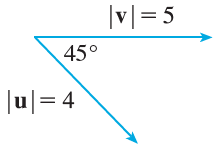
\includegraphics[scale = 1.25]{124_1.png}
		\end{flushleft}
		
			\vs{1}
			\newpage
			
	\subsubsection*{Properties of the Cross Product}	
		\begin{rmk}[Properties of the Cross Product]
			If $\textbf{a}$, $\textbf{b}$, and $\textbf{c}$ are vectors and $k$ is a scalar, then\\[15pt]
			\begin{itemize}
				\setlength\itemsep{15pt}
				\item $\textbf{a}\times \textbf{b} = $\blank{2}
				\item $(k\textbf{a})\times \textbf{b} = $\blank{4}
				\item $\textbf{a}\times (\textbf{b} + \textbf{c}) = $\blank{3}
				\item $(\textbf{a}+\textbf{b}) \times \textbf{c} = $\blank{3}
				\item $\textbf{a}\cdot (\textbf{b}\times \textbf{c}) = $\blank{2}
				\item $\textbf{a}\times (\textbf{b}\times\textbf{c}) = $\blank{3}
			\end{itemize}
		\end{rmk}
		
		\begin{ex}
			Use properties of cross products to help compute the following:
			\begin{enumerate}[(a)]
				\item $(\textbf{i}\times\textbf{j})\times\textbf{k}$
					\vs{1}
					
				\item $\textbf{k}\times (\textbf{i}-2\textbf{j})$
					\vs{1}
					
				\item $(\textbf{j}-\textbf{k})\times (\textbf{k}-\textbf{i})$
					\vs{1}
			\end{enumerate}
		\end{ex}
			\newpage
			
		\begin{ex}
			Prove the the third property of cross products.
		\end{ex}
			\vs{1}
			
	\subsubsection*{Applications}
		\begin{defn}[Scalar Triple Product]
			Given three vectors $\textbf{a}, \textbf{b},$ and \textbf{c}, the \textbf{scalar triple product} of the vectors is the quantity\\[15pt]
				\[\textbf{a}\cdot (\textbf{b}\times \textbf{c}) = \hspace{3in}\]
		\end{defn}
		
		\begin{rmk}[Meaning of Scalar Triple Product]
			The magnitude of the scalar triple product, $|\textbf{a}\cdot (\textbf{b}\times \textbf{c})|$, gives \blank{1.5}\\[15pt] \blank{3}.
		\end{rmk}
		
		\begin{ex}
			Find the volume of the parallelepiped determined by the vectors $\textbf{a} = \lrangle{1,2,3}$, $\textbf{b} = \lrangle{-1,1,2}$, and $\textbf{c} = \lrangle{2,1,4}$.
		\end{ex}
			\vs{1}
			\newpage
			
		\begin{ex}
			Use the scalar triple product to show that the vectors $\textbf{a} = \lrangle{1,4,-7}$, $\textbf{b} = \lrangle{2,-1,4}$, and $\textbf{c} = \lrangle{0,-9,18}$ are \emph{coplanar}, i.e. they lie in the same plane.
		\end{ex}
			\vs{1}
			
		\begin{defn}[Torque]
			The \textbf{torque} $\mathbf{\tau}$ created by a force \textbf{F} acting on a rigid body at a point given by the position\\[15pt] vector $\textbf{r}$ is \blank{2.5}.  Torque measures the tendency of a body to rotate about the origin.
		\end{defn}
		
		\begin{ex}
			A bolt is tightened by applying a 60 N force to a 0.2 meter wrench.  The angle between the wrench and the force vector is $45\dc$.  Find the torque on the wrench, and then the magnitude of the torque vector.
		\end{ex}
			\vs{1}
			
			\newpage
			
	\subsection*{After Class Activities}
		\begin{ex}
			Find a nonzero vector orthogonal to the plane through the points given.
			\begin{enumerate}[(a)]
				\item $P(1,0,1)$, $Q(-2,1,3)$, $R(4,2,5)$
					\vs{1}
					
				\item $P(0,0,-3)$, $Q(4,2,0)$, $R(3,3,1)$
					\vs{1}
			\end{enumerate}
		\end{ex}
		
		\begin{ex}
			Use the scalar triple product to verify that the vectors $\textbf{u} = \lrangle{1,5,-2}$, $\textbf{v} = \lrangle{3,-1,0}$ and $\textbf{w} = \lrangle{5,9,-4}$ are coplanar.
		\end{ex}
			\vs{1}
			\newpage
			
		\begin{ex}
			A bicycle pedal is pushed by a foot with a 60 N force as shown below.  The shaft of the pedal is 18 cm long.  Find the magnitude of the torque about $P$.
		\end{ex}\\
		\begin{flushleft}
			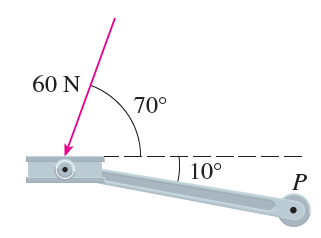
\includegraphics[scale = .75]{124_2.png}
		\end{flushleft}
			\vs{1}
			
		\begin{ex}
			Show that $|\textbf{a}\times \textbf{b}|^2 = |\textbf{a}|^2|\textbf{b}|^2 - (\textbf{a}\cdot\textbf{b})^2$
		\end{ex}
			\vs{1}
	
\clearpage
\end{document}
